\begin{frame}
\frametitle{Le Projet}

\textbf{Choix du jeu :}
\begin{itemize}
    \item Jeu combinatoire abstrait
    \item À deux joueurs
    \item À information complète et parfaite
\end{itemize}

\bigskip

\textbf{Objectifs techniques :}
\begin{itemize}
    \item Implémentation d’une version \textbf{Joueur vs Joueur}
    \item Conception d’une IA avec l’algorithme \textbf{Minimax}
    \item Optimisation grâce à l’\textbf{élagage alpha-bêta}
\end{itemize}
\end{frame}


\begin{frame}
\frametitle{Choix techniques}
\begin{itemize}
    \item Jeu Othello (aussi appelé Reversi)
    \item Codé en Python avec séparation Modèle / Vue
    \item Utilisation de Minimax avec une fonction d’évaluation multi-critères
    \item Critères inspirés des stratégies d’Othello
\end{itemize}
\end{frame}

\begin{frame}
\frametitle{Présentation du jeu Othello}

\begin{columns}
    \begin{column}{0.65\textwidth}
        \begin{itemize}
            \item Plateau de $8 \times 8$
            \item Deux joueurs : Noir et Blanc
            \item Le but est d’avoir un maximum de pions à la fin
        \end{itemize}
    \end{column}
        \bigskip    
    \begin{column}{0.35\textwidth}
        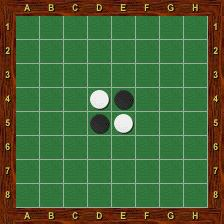
\includegraphics[width=\linewidth]{img/debut-othello.jpg}
    \end{column}
\end{columns}
\end{frame}

\begin{frame}
\frametitle{Présentation du jeu Othello}
\begin{columns}
    \begin{column}{0.65\textwidth}
        \begin{itemize}
            \item Plateau de $8 \times 8$
            \item Deux joueurs : Noir et Blanc
            \item Le but est d’avoir un maximum de pions à la fin
        \end{itemize}
        \bigskip
        \textbf{Déroulement :}
        \begin{itemize}
            \item Le joueur Noir commence
            \item Chaque joueur joue à tour de rôle
            \item La partie se termine quand plus aucun coup n’est possible
        \end{itemize}
    \end{column}
    
    \begin{column}{0.35\textwidth}
        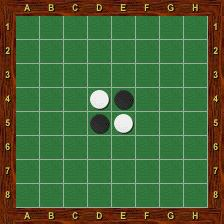
\includegraphics[width=\linewidth]{img/debut-othello.jpg}
    \end{column}
\end{columns}
\end{frame}

\begin{frame}
\frametitle{La pose d’un pion}

\begin{columns}
    \begin{column}{0.65\textwidth}
        \begin{itemize}
            \item Un pion est posé sur une \textbf{case vide} de l’othellier, \textbf{adjacente} à un pion adverse
            \item Il doit \textbf{encadrer un ou plusieurs pions adverses} entre ce nouveau pion et un autre pion de la même couleur déjà présent sur le plateau
            \item En jaune sur l’image : les cases où le joueur noir peut jouer
        \end{itemize}    
    \end{column}
    
    \begin{column}{0.35\textwidth}
        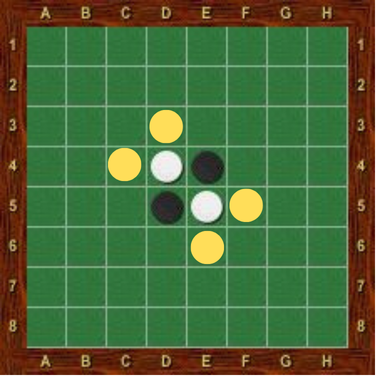
\includegraphics[width=\linewidth]{img/othello-coup-possible.png}
    \end{column}
\end{columns}

\end{frame}

\begin{frame}
\frametitle{Stratégies de base}

Quelques principes stratégiques fondamentaux d’Othello :
\vspace{1em}
\begin{columns}
    \begin{column}{0.65\textwidth}
        \begin{itemize}
            \item \textbf{Capturer un maximum de pions}
            \vspace{0.5em}
        
            \item \textbf{Contrôler les coins} (en vert)
            \vspace{0.5em}
        
            \item \textbf{Occuper les bords} (en bleu)
            \vspace{0.5em}
         
            \item \textbf{Réduire la mobilité adverse}
            \vspace{0.5em}
           
            \item \textbf{Éviter les cases adjacentes aux coins}(en rouge)
        \end{itemize}
    \end{column} 
    \begin{column}{0.35\textwidth}
        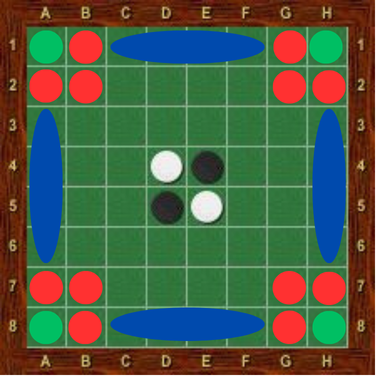
\includegraphics[width=\linewidth]{img/othello-strategie-de-base.png}
    \end{column}
\end{columns}
\end{frame}

\begin{frame}
\frametitle{L’algorithme Minimax — Principe}

\textbf{Objectif :} prendre la meilleure décision possible.

\begin{itemize}
    \item Construire un \textbf{arbre de décision}.
    \item L’IA joue en tant que \textbf{Max}, l’adversaire en tant que \textbf{Min}.
    \item Évaluer chaque position à l’aide d’une \textbf{fonction d'évaluation}.
    \item \textbf{Profondeur dynamique :} la profondeur de l’arbre est adaptée au stade de la partie.
\end{itemize}

\begin{center}
    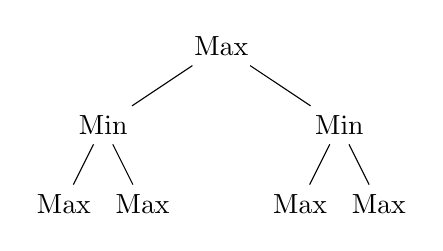
\begin{tikzpicture}[level distance=1cm,
      level 1/.style={sibling distance=3cm},
      level 2/.style={sibling distance=1cm}]
        \node {Max}
            child {node {Min}
                child {node {Max}}
                child {node {Max}}
            }
            child {node {Min}
                child {node {Max}}
                child {node {Max}}
            };
    \end{tikzpicture}
\end{center}

\end{frame}

\begin{frame}
\frametitle{L’algorithme Minimax — Avantages et limites}

\textbf{Pourquoi utiliser Minimax ?}

\begin{itemize}
    \item Anticipe les \textbf{réactions de l’adversaire}.
    \item Évite les \textbf{pièges à court terme}.
    \item Permet de simuler un \textbf{comportement stratégique et réfléchi}.
\end{itemize}

\vspace{1em}
\textbf{Limite principale :} le coût en \textbf{temps de calcul} augmente fortement avec la profondeur.

\begin{block}{Solution}
Utilisation de l’\textbf{élagage alpha-bêta} pour ignorer des branches non pertinentes de l’arbre.
\end{block}
\end{frame}
